% Options for packages loaded elsewhere
\PassOptionsToPackage{unicode}{hyperref}
\PassOptionsToPackage{hyphens}{url}
\PassOptionsToPackage{dvipsnames,svgnames,x11names}{xcolor}
%
\documentclass[
  letterpaper,
  DIV=11,
  numbers=noendperiod]{scrartcl}

\usepackage{amsmath,amssymb}
\usepackage{iftex}
\ifPDFTeX
  \usepackage[T1]{fontenc}
  \usepackage[utf8]{inputenc}
  \usepackage{textcomp} % provide euro and other symbols
\else % if luatex or xetex
  \usepackage{unicode-math}
  \defaultfontfeatures{Scale=MatchLowercase}
  \defaultfontfeatures[\rmfamily]{Ligatures=TeX,Scale=1}
\fi
\usepackage{lmodern}
\ifPDFTeX\else  
    % xetex/luatex font selection
\fi
% Use upquote if available, for straight quotes in verbatim environments
\IfFileExists{upquote.sty}{\usepackage{upquote}}{}
\IfFileExists{microtype.sty}{% use microtype if available
  \usepackage[]{microtype}
  \UseMicrotypeSet[protrusion]{basicmath} % disable protrusion for tt fonts
}{}
\makeatletter
\@ifundefined{KOMAClassName}{% if non-KOMA class
  \IfFileExists{parskip.sty}{%
    \usepackage{parskip}
  }{% else
    \setlength{\parindent}{0pt}
    \setlength{\parskip}{6pt plus 2pt minus 1pt}}
}{% if KOMA class
  \KOMAoptions{parskip=half}}
\makeatother
\usepackage{xcolor}
\setlength{\emergencystretch}{3em} % prevent overfull lines
\setcounter{secnumdepth}{-\maxdimen} % remove section numbering
% Make \paragraph and \subparagraph free-standing
\ifx\paragraph\undefined\else
  \let\oldparagraph\paragraph
  \renewcommand{\paragraph}[1]{\oldparagraph{#1}\mbox{}}
\fi
\ifx\subparagraph\undefined\else
  \let\oldsubparagraph\subparagraph
  \renewcommand{\subparagraph}[1]{\oldsubparagraph{#1}\mbox{}}
\fi


\providecommand{\tightlist}{%
  \setlength{\itemsep}{0pt}\setlength{\parskip}{0pt}}\usepackage{longtable,booktabs,array}
\usepackage{calc} % for calculating minipage widths
% Correct order of tables after \paragraph or \subparagraph
\usepackage{etoolbox}
\makeatletter
\patchcmd\longtable{\par}{\if@noskipsec\mbox{}\fi\par}{}{}
\makeatother
% Allow footnotes in longtable head/foot
\IfFileExists{footnotehyper.sty}{\usepackage{footnotehyper}}{\usepackage{footnote}}
\makesavenoteenv{longtable}
\usepackage{graphicx}
\makeatletter
\def\maxwidth{\ifdim\Gin@nat@width>\linewidth\linewidth\else\Gin@nat@width\fi}
\def\maxheight{\ifdim\Gin@nat@height>\textheight\textheight\else\Gin@nat@height\fi}
\makeatother
% Scale images if necessary, so that they will not overflow the page
% margins by default, and it is still possible to overwrite the defaults
% using explicit options in \includegraphics[width, height, ...]{}
\setkeys{Gin}{width=\maxwidth,height=\maxheight,keepaspectratio}
% Set default figure placement to htbp
\makeatletter
\def\fps@figure{htbp}
\makeatother

\usepackage{booktabs}
\usepackage{longtable}
\usepackage{array}
\usepackage{multirow}
\usepackage{wrapfig}
\usepackage{float}
\usepackage{colortbl}
\usepackage{pdflscape}
\usepackage{tabu}
\usepackage{threeparttable}
\usepackage{threeparttablex}
\usepackage[normalem]{ulem}
\usepackage{makecell}
\usepackage{xcolor}
\KOMAoption{captions}{tableheading}
\makeatletter
\@ifpackageloaded{caption}{}{\usepackage{caption}}
\AtBeginDocument{%
\ifdefined\contentsname
  \renewcommand*\contentsname{Table of contents}
\else
  \newcommand\contentsname{Table of contents}
\fi
\ifdefined\listfigurename
  \renewcommand*\listfigurename{List of Figures}
\else
  \newcommand\listfigurename{List of Figures}
\fi
\ifdefined\listtablename
  \renewcommand*\listtablename{List of Tables}
\else
  \newcommand\listtablename{List of Tables}
\fi
\ifdefined\figurename
  \renewcommand*\figurename{Figure}
\else
  \newcommand\figurename{Figure}
\fi
\ifdefined\tablename
  \renewcommand*\tablename{Table}
\else
  \newcommand\tablename{Table}
\fi
}
\@ifpackageloaded{float}{}{\usepackage{float}}
\floatstyle{ruled}
\@ifundefined{c@chapter}{\newfloat{codelisting}{h}{lop}}{\newfloat{codelisting}{h}{lop}[chapter]}
\floatname{codelisting}{Listing}
\newcommand*\listoflistings{\listof{codelisting}{List of Listings}}
\makeatother
\makeatletter
\makeatother
\makeatletter
\@ifpackageloaded{caption}{}{\usepackage{caption}}
\@ifpackageloaded{subcaption}{}{\usepackage{subcaption}}
\makeatother
\ifLuaTeX
  \usepackage{selnolig}  % disable illegal ligatures
\fi
\usepackage{bookmark}

\IfFileExists{xurl.sty}{\usepackage{xurl}}{} % add URL line breaks if available
\urlstyle{same} % disable monospaced font for URLs
\hypersetup{
  pdftitle={Documento devolución colegios},
  pdfauthor={Equipo Edumer},
  colorlinks=true,
  linkcolor={blue},
  filecolor={Maroon},
  citecolor={Blue},
  urlcolor={Blue},
  pdfcreator={LaTeX via pandoc}}

\title{Documento devolución colegios}
\author{Equipo Edumer}
\date{}

\begin{document}
\maketitle

\subsection{Introducción}\label{introducciuxf3n}

Se estructurá de acuerdo a tres grandes módulos

Esta es la idea para cuando tengamos todos los datos.

\subsection{Reporte metodológico}\label{reporte-metodoluxf3gico}

\subsection{1. Meritocracia}\label{meritocracia}

\subsubsection{1.1. Meritocracia en la
sociedad}\label{meritocracia-en-la-sociedad}

\paragraph{1.1.1. Creencias en la
meritocracia}\label{creencias-en-la-meritocracia}

\subparagraph{Percepciones}\label{percepciones}

\begin{itemize}
\tightlist
\item
  Respecto a criterios de mérito individual
\end{itemize}

\textbf{Esfuerzo} en la sociedad chilena:

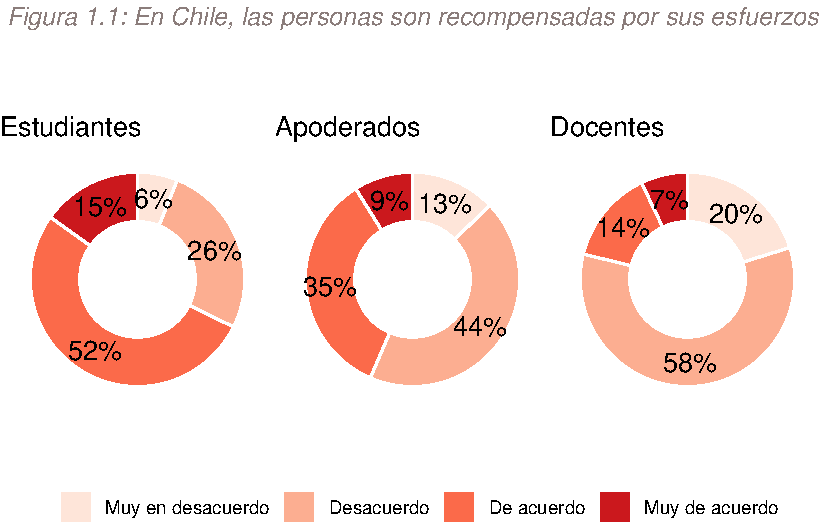
\includegraphics{doc-colegios-con-profes-y-apoderados_files/figure-pdf/unnamed-chunk-6-1.pdf}

En primer lugar, se observan claras diferencias entre adultos y
estudiantes. Tanto profesores como apoderados estan en desacuerdo con la
frase y, específicamente, los apoderados están más de acuerdo que los
docentes. Así, los estudiantes parecen estar más de acuerdo con que las
personas en el país son recompensadas por sus esfuerzos (52\%). Aún así,
ninguno de los tres actores esta muy de acuerdo con este criterio de
mérito individual.

\textbf{Talento} (inteligencia y habilidad) en la sociedad chilena:

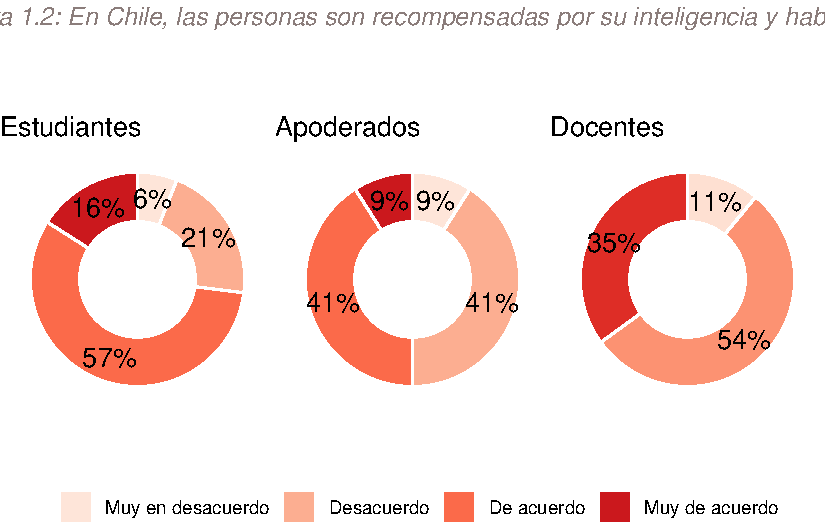
\includegraphics{doc-colegios-con-profes-y-apoderados_files/figure-pdf/unnamed-chunk-7-1.pdf}

Si bien los tres actores están de acuerdo con la frase y, por ende,
creen en el mérito en base al talento, los docentes están más de acuerdo
con la afirmación. Acumulando el 89\% de sus respuestas en las
categorías ``Muy de acuerdo'' y ``De acuerdo''.

\begin{itemize}
\tightlist
\item
  Respecto al \textbf{mérito} en la sociedad chilena:
\end{itemize}

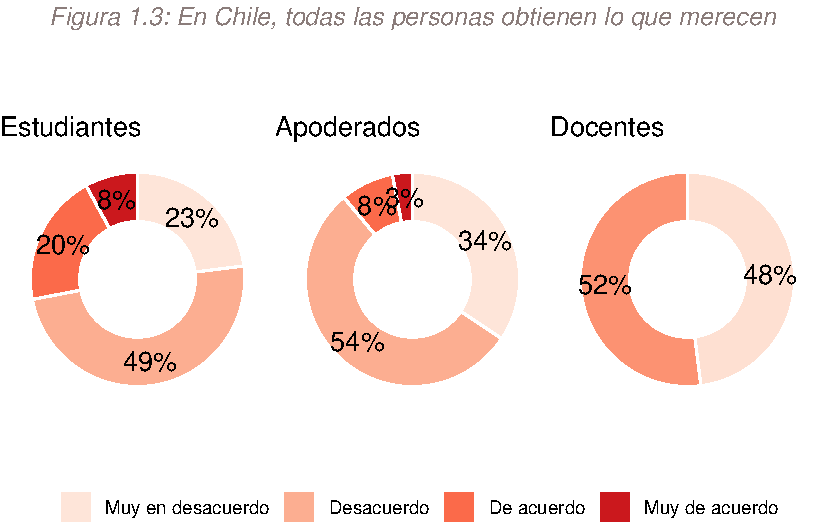
\includegraphics{doc-colegios-con-profes-y-apoderados_files/figure-pdf/unnamed-chunk-9-1.pdf}

Los docentes se muestran en desacuerdo en su totalidad con la idea de
que las personas son recompensadas por sus méritos en la sociedad
chilena. Si bien estudiantes y apoderados también se muestran en su
mayoría en desacuerdo, los estudiantes presentan un 20\% de acuerdo con
la afirmación.

En vista de las diferencias entre estudiantes, apoderados y docentes, se
presentará la forma en que se distribyen estas creencias de acuerdo a
sus \textbf{caracteristicas sociodemográficas más relevantes}.

En concordancia con la preodminante creencia en la meritocracia de
las/los estudiantes, a continuación se observa cómo se expresan dichas
creencias conforme al \textbf{curso} en que se encuentran:

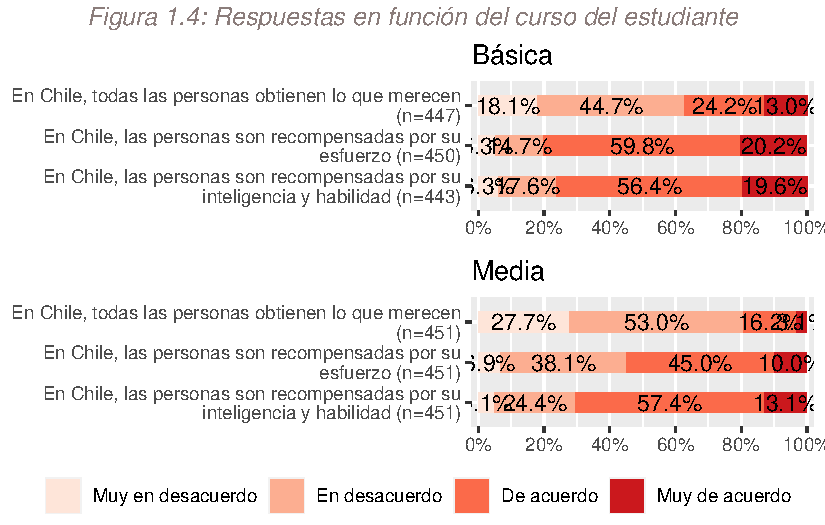
\includegraphics{doc-colegios-con-profes-y-apoderados_files/figure-pdf/unnamed-chunk-11-1.pdf}

Estudiantes de educación básica estan más de acuerdo con ambos criterios
individuales de meritocracia en la sociedad que los estudiantes de
educación media.

Además, a propósito del predominante desacuerdo de las/los docentes
frente a los criterios de mérito individual en la sociedad, se muestra
cómo se dsitribuyen estas creencias en función de su \textbf{género}:

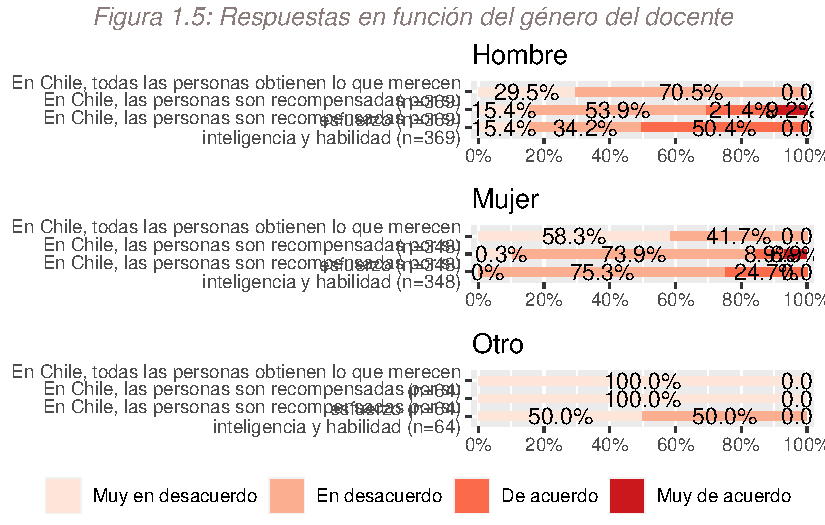
\includegraphics{doc-colegios-con-profes-y-apoderados_files/figure-pdf/unnamed-chunk-13-1.pdf}

Mujeres y otras identidades sexogenéricas están en desacuerdo con la
frase sobre el mérito social y con ambos criterios de mérito individual.
Contrariamente, los docentes hombres están de acuerdo en un 50.4\% con
la afirmación sobre el talento en la sociedad.

En cuanto a la distribución por \textbf{género} de los apoderados, se
observa lo siguiente:

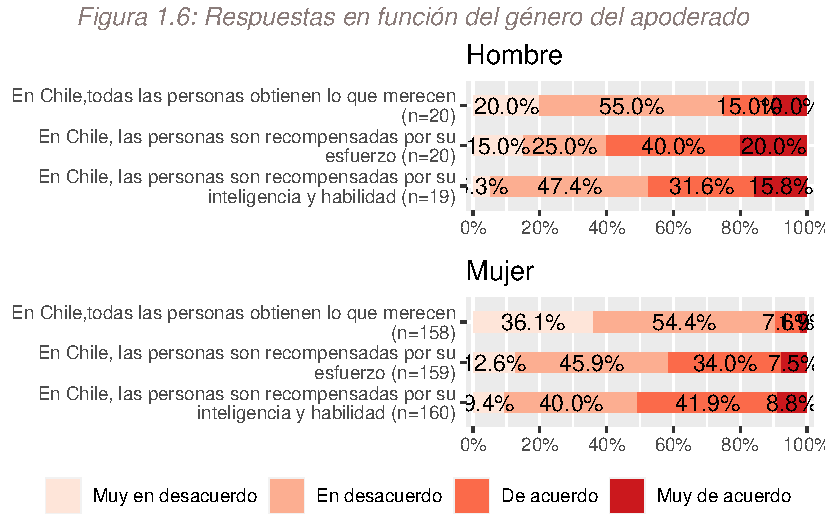
\includegraphics{doc-colegios-con-profes-y-apoderados_files/figure-pdf/unnamed-chunk-15-1.pdf}

Las apoderadas están más de acuerdo con el mérito en base al talento en
la sociedad y los apoderados con el mérito en base al esfuerzo.

\begin{itemize}
\tightlist
\item
  Respecto a factores no meritocráticos
\end{itemize}

Estos factores aluden a externalidades del mérito individual como la
herencia, los contactos y la suerte. Por ello, se presentan preguntas
referidas a la percepción respecto a los logros individuales de las
personas que tienen padres ricos, buenos contactos y mejores
oportunidades en la vida.

\textbf{Padres ricos}

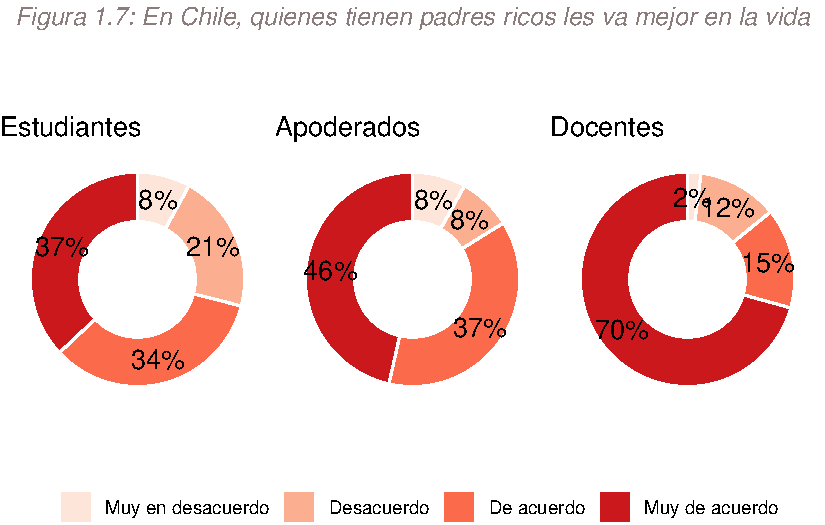
\includegraphics{doc-colegios-con-profes-y-apoderados_files/figure-pdf/unnamed-chunk-17-1.pdf}

\textbf{Buenos contactos}

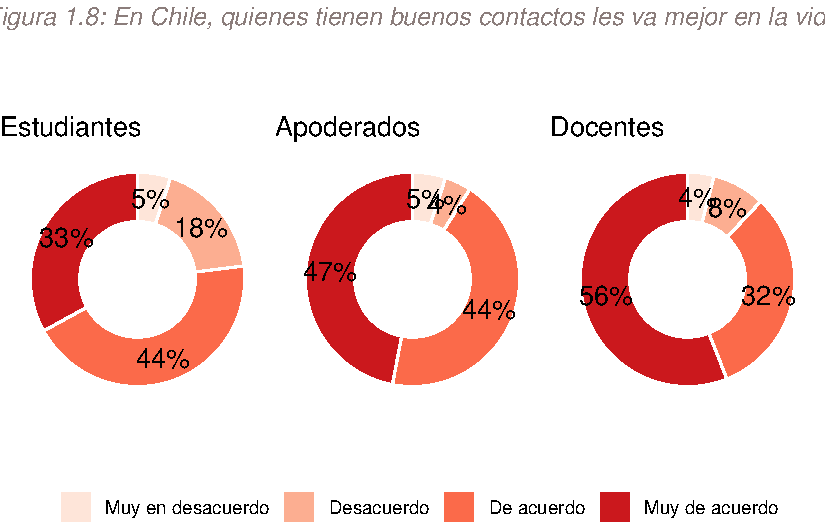
\includegraphics{doc-colegios-con-profes-y-apoderados_files/figure-pdf/unnamed-chunk-19-1.pdf}

\textbf{Oportunidades}

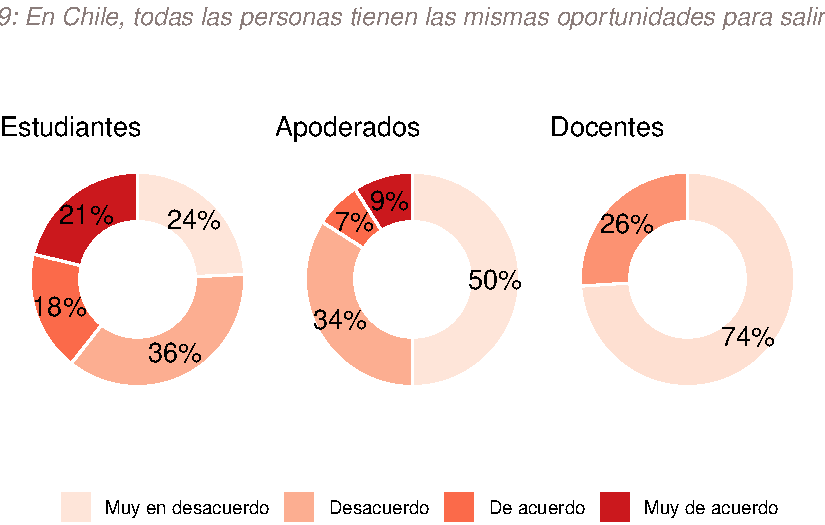
\includegraphics{doc-colegios-con-profes-y-apoderados_files/figure-pdf/unnamed-chunk-21-1.pdf}

\subparagraph{Preferencias}\label{preferencias}

\subsubsection{1.2. Meritocracia en la
escuela}\label{meritocracia-en-la-escuela}

\paragraph{1.2.1. Creencias en la
meritocracia}\label{creencias-en-la-meritocracia-1}

\subparagraph{Percepciones}\label{percepciones-1}

\subparagraph{Preferencias}\label{preferencias-1}

\paragraph{1.2.2 Justicia en la notas}\label{justicia-en-la-notas}

\subsection{2. Ciudadania}\label{ciudadania}

\subsubsection{2.1. Formacióm ciudadana en la
escuela}\label{formaciuxf3m-ciudadana-en-la-escuela}

\paragraph{2.1.1. Percepción respecto a la importancia que le entrega la
escuela}\label{percepciuxf3n-respecto-a-la-importancia-que-le-entrega-la-escuela}

\paragraph{2.1.2. En el espacio de
clases}\label{en-el-espacio-de-clases}

\subsubsection{2.2. Participación
política}\label{participaciuxf3n-poluxedtica}

\paragraph{2.2.1. Participación política
actual}\label{participaciuxf3n-poluxedtica-actual}

\paragraph{2.2.2. Participación política
futura}\label{participaciuxf3n-poluxedtica-futura}

\subsubsection{2.3. Buena ciudadanía}\label{buena-ciudadanuxeda}

\subsubsection{}\label{section}



\end{document}
